\documentclass{llncs}

% For FIGURES: (1) include figures and (2) float position of figures
\usepackage{graphicx}
\usepackage{subfigure,dblfloatfix} %to fix the problem of [h!] [t!] [!b]

% For TABLES: (1) columns with predefined width (2) to make colored cells
\usepackage{array} 
\newcolumntype{L}[1]{>{\raggedright\let\newline\\\arraybackslash\hspace{0pt}}m{#1}}
\newcolumntype{C}[1]{>{\centering\let\newline\\\arraybackslash\hspace{0pt}}m{#1}}
\newcolumntype{R}[1]{>{\raggedleft\let\newline\\\arraybackslash\hspace{0pt}}m{#1}}
\usepackage[]{colortbl}

\usepackage{bbding}
\usepackage{pifont}
\usepackage{wasysym}
\usepackage{amssymb}

\begin{document}

\title{\huge DDoS Filtering Tool\\ \small A Design Paper}

\author{Jos\'e Jair Santanna \and Julik Keijer}
\institute{University of Twente, the Netherlands\\
\email{j.j.santanna@utwente.nl \& keijerjs@gmail.com},\\ 
\texttt{http://ddosdb.org/ddosfiltering}}
\maketitle             

%\begin{abstract}
%\end{abstract}

\section{Introduction}

\section{Collaborators Requirement}

\noindent
\textsc{Main requirement:} 
\begin{itemize}
	\item Facilitate the removing of any private information that can be potentially used for identifying either the collaborators or their clients;
	\item Generate a summary of the attack and the IP addresses that are involved in the attack;
	\item Generate a new network file with only the attack records.
\end{itemize}

\noindent
\textsc{Additional requirements:}
\begin{itemize}
	\item Process the traffic at the collaborators' infrastructure to avoid leak of information;
	\item Facilitated the deployment of the filtering tool; 
	\item Speedup the loading process of visualizations;
	\item Create simple and meaningful visualizations;
	\item Have a dynamic (and manual) filtering interface;
	\item Highlight outliers.
\end{itemize}

\section{Tasks \& Modules}

The steps needed to achieve the main requirement are the following:
\begin{enumerate}
	\item Receive an uploaded network file that contains a DDoS attack (pcap[ng] or nfdump types);	
	\item Pre-filter the uploaded network file keeping only the ingress traffic;
	\item Highlight the potential attack targets, i.e., the destination IP addresses that received more network traffic);
	\item Highlight the IP protocol that generates more network traffic towards the highlighted destination IP address;
	\item Present summarized information of source IPs that sent traffic using the highlighted IP protocol;
	\item Highlight (and manually remove) the source IPs that does not follow an attack pattern (outliers);
	\item Classify the set of remaining source IPs as a type of DDoS attack;
	\item[*8.] Use the set of remaining source IPs to filter the pre-filtered traffic (output of step 2) towards identify multi-vector attacks;  
	\item[9.] Repeat steps 3, 4, 5 and 6 until the collaborator is satisfied about the remaining information;
	\item[10.] Generate a new network attack file with only the remaining information;
	\item[11.] Export the new network attack file and the summary of the attack to DDoSDB.
\end{enumerate}

\begin{figure}[!ht] 
\centering 
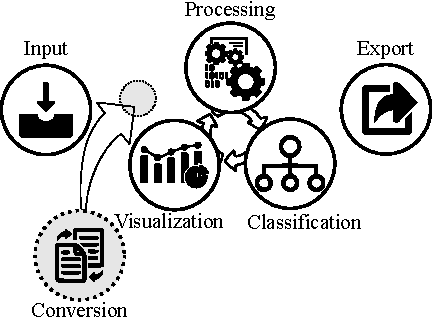
\includegraphics[]{figs/modules.pdf}
\caption{DDoS filtering tool modules.} 
\label{fig:modules} 
\end{figure}


\begin{table}[h!] \small \center \caption{Attack information shared by
initiative.}
\label{tab:attack_fields} \begin{tabular}{|c| l | c |c|c|c|c|c|} \hline
&\textbf{Information}      & \textbf{Obtained}&\cite{digitalattackmap2013web} &
\cite{norse2015web}& \cite{ipew2015web}  & \cite{fireeye2015web} &
\cite{kaspersky2015web2}\\ \hline

1&Start time 	&field&  $\checkmark$	& $\checkmark$	& ~
& ~ & ~    \\ \hline    
2&Duration 		&field*& $\checkmark$	& ~ & ~
& ~ & ~   \\ \hline 
3&Max bit rate	&field*& $\checkmark$	& ~ & ~ & ~ & ~
\\ \hline 
4&Src.  port 		&field& $\checkmark$	& ~ & ~ & ~ & ~   \\\hline 
5&Dst.  port &field& $\checkmark$	& $\checkmark$	& ~ & ~ & $\checkmark$
\\ \hline 
6&Attack type&heuristic& $\checkmark$ & $\checkmark$	&
$\checkmark$ &~ & $\checkmark$    \\ \hline \hline\hline 
7&Src.  IP &field& ~ &
$\checkmark$ & $\checkmark$& ~ & ~    \\ \hline 
8&Src. IP country	&enrich&
$\checkmark$ & $\checkmark$ & $\checkmark$& $\checkmark$ & $\checkmark$   \\
\hline    
9&Src.  IP city &enrich& ~ & $\checkmark$	& ~ & ~ & ~   \\  \hline
10&Src. IP ASN &enrich& ~ & $\checkmark$	& ~ & ~ & ~ \\ \hline \hline\hline
\rowcolor{red}11&Dst.  IP &field& ~ & ~ & $\checkmark$& ~ & ~ \\\hline
12&Dst. IP country&enrich& $\checkmark$ & $\checkmark$	& $\checkmark$& $\checkmark$ & ~
\\ \hline \rowcolor{red}13&Dst. IP City &enrich& ~ & $\checkmark$	& ~ & ~ & ~   \\
\hline \rowcolor{red}14&Dst. IP ASN &enrich& ~ & $\checkmark$ & ~ & ~ & ~ \\ \hline
\end{tabular} \end{table}

\begin{table}[h!] \small \center \caption{Missing attack information.}
\label{tab:missing_info} \begin{tabular}{| c | l |c|} \hline
&\textbf{Information}     & \textbf{Obtained}\\ 
\hline 
1& Packet peak rate & field*\\ \hline
2&\# Src. IPs &field*\\\hline	
3&\# restricted Src. IPs & enrich \\\hline 
4&\# Src. IPs with fragm. & field \\\hline
5&Attack responsible (blame)& manual\\\hline
\hline\hline
6&Src. IP \# total packets&field\\ \hline
7&Src. IP \# frag. packets  &field\\ \hline 
8&Src. IP data rate & field*\\ \hline
9&Src. IP packet rate & field* \\ \hline
%10&Src. IP traffic duration& field* \\\hline
10&Src. IP restricted?  &enrich \\ \hline 
11&Src. IP packet length &field \\ \hline 
12&Src. IP TTL  &field \\ \hline
\rowcolor{yellow}13&Src. IP TCP flags &field \\ \hline 
\rowcolor{yellow}15&Src. IP HTTP payload* & field\\ \hline
\rowcolor{yellow}14&Src. IP DNS query  & field\\ \hline 
\rowcolor{yellow}16&Src. IP open ports &enrich\\ \hline 

\end{tabular}
\end{table}


Web-based that performs offline filtering;




\section{Preliminary results}
\end{document}
